%!TEX root = ../thesis.tex

\chapter{A Comparative Study of AC and DC Electric Vehicle Charging Station Usage}
\label{ch:charging}

\ifpdf
	\graphicspath{{Chapter10/Figs/Raster/}{Chapter10/Figs/PDF/}{Chapter10/Figs/}}
\else
	\graphicspath{{Chapter10/Figs/Vector/}{Chapter10/Figs/}}
\fi

Fast-DC charging stations can charge an Electric Vehicle (EV) several times faster than Level-2 AC charging stations. Using a network of DC charging stations, it becomes possible to use EVs for long distance, cross-country driving with only short recharging stops. This paper examines and compares typical customer usage patterns at DC fast-charging stations (50 kW) versus Level-2 AC stations (7 kW). It includes data collected from the University of Western Australia's AC and DC charging network in the Perth metropolitan area, as well as from stations along the highway connecting Perth to Augusta in the rural South West of Western Australia (over 300 km apart). A cost model is also drawn up to calculate the operating cost and break-even requirement across several different styles of charging stations. User behaviour and adoption of certain charging infrastructure is crucial for the take up of electric vehicles in general. EV charging standards and infrastructure availability have, therefore, a fundamental influence on the electrification of transport.

\section{Introduction}
\label{sec:10:intro}
Electric vehicles (EVs) are an environmentally friendly alternative to traditional internal combustion engine vehicles (ICE), which are a major contributor of carbon emissions~\cite{department_of_infrastructure_and_regional_development_vehicle_2016}. EVs are emission free if charged from renewable energy sources and they improve urban air quality as well as fuel security~\cite{climateworks_australia_path_2016}. Additionally, they are becoming more and more common on the roads today, with an increase on the roads worldwide from 100,000 vehicles in 2012 to over 1 million in 2016~\cite{statista_worldwide_nodate}. This paper discusses the data collected from three different sources --- the Western Australian Electric Vehicle Trial~\cite{mader_western_2013}, The University of Western Australia’s fast-charging station~\cite{noauthor_electric_2017} and the RAC-funded Electric Highway in Western Australia~\cite{rac_wa_rac_nodate}. Comparing these trials allows the assessment of different charging infrastructure types, different locations and different usage patterns between paying and non-paying customers (e.g. free stations). The current state of EV charging technology,  specifically international standards and their adoption in different countries, is also examined by using publicly available information~\cite{plugshare_plugshare_nodate}. Electric vehicle adoption has a direct link to the availability of fast-charging infrastructure~\cite{gebauer_changing_2016} (though not without contention~\cite{bailey_is_2015}). The infrastructure installation and maintenance of these charging stations is an expensive process, so having greater clarity on usage patterns can assist organisations in their decision making.

This paper’s aim is to give an overview of all charging infrastructure developed to date and the overall necessity of an electric vehicle charging station network. The University of Western Australia's Renewable Energy Vehicle Project (REV) installed Western Australia's first EV charging infrastructure in 2010 as a series of 23 Level-2 (``medium fast'') AC charging stations (7.7 kW), funded through the WA Electric Vehicle Trial in combination with an ARC Linkage grant~\cite{mader_western_2013}. REV later installed Australia's first commercial CCS fast-DC charging station (50 kW) in 2014.

\nomenclature[z-arc]{ARC}{Australian Research Council}

Although the EV Trial and REV/UWA had proposed an Electric Highway through Western Australia with several partners, it took over two years until RAC WA eventually funded this network. Funds were given to nine rural communities to install a pair of AC and DC charging stations at each location, plus a tenth at the RAC headquarters in West Perth. The rural locations are Mandurah, Harvey, Bunbury, Busselton, Dunsborough, Margaret River, Augusta, Donnybrook and Nannup. While power is provided free of charge at all UWA stations, users of the Electric Highway have to pay \$0.50 per kWh. This is twice the amount of the domestic energy rate, which makes these stations unattractive to local EV owners.

The remainder of this paper is organised as follows. Section~\ref{sec:10:acdc} presents the various types of EV charging infrastructure from a global to local standpoint. Section~\ref{sec:10:evcharging} explores different EV charging methods and the preferred methods of adoption. Section~\ref{sec:10:analysis} analyses and compares data collected from the UWA AC and DC charging stations, and the local Electric Highway network. In Section~\ref{sec:10:cost}, a cost model then drawn using this data from the UWA stations. The data analysis is validated in Section~\ref{sec:10:validation} using a similar study before a summary and concluding remarks are drawn in Section~\ref{sec:10:conclu}.

\section{AC and DC Charging Infrastructure}
\label{sec:10:acdc}
Countries around the world have adopted different charging standards, and in some cases more than one. The United States and Canada have passed legislation to adopt the IEC 62196 Type-1 standard (single-phase AC), while the European Union has adopted the IEC 62196 Type-2 charging standard (three-phase AC). For DC, these countries use the compatible Combined Charging System (CCS) standard, again as Type-1 (USA, Canada) and Type-2 (Europe), which allows vehicle manufacturers to use a single combined vehicle inlet for either AC or DC charging. France and Italy initially adopted Type-3 (Scame) connectors and are currently in transition towards Type-2 connectors. 

Japan uses almost exclusively its CHAdeMO standard for DC charging, while China uses its GB/T standard. Some countries, like Australia, have failed to adopt any national standard and then had to suffer the consequences. A mix of Type-1 and Type-2 charging stations were installed in different states in Australia initially when mostly Type-1 vehicles were imported into the country (no EVs were ever produced in Australia). This changed in late 2017, when leading vehicle manufacturers decided to change over to Type-2 for newly imported vehicles, and other manufacturers can be presumed to follow. This leads to presumptions that the whole country should adopt Type-2 stations as a standard which would cause major problems for both charging station operators, as they could not serve all cars (unless they installed Type-2 stations, which have exchangeable power cables), and vehicle owners, who would not be able to charge their cars on CCS stations of the wrong type. Using Type-2 chargers, however, makes sense for Australia, as the country does have a three-phase power grid.

\begin{figure}[H]
	\centering
	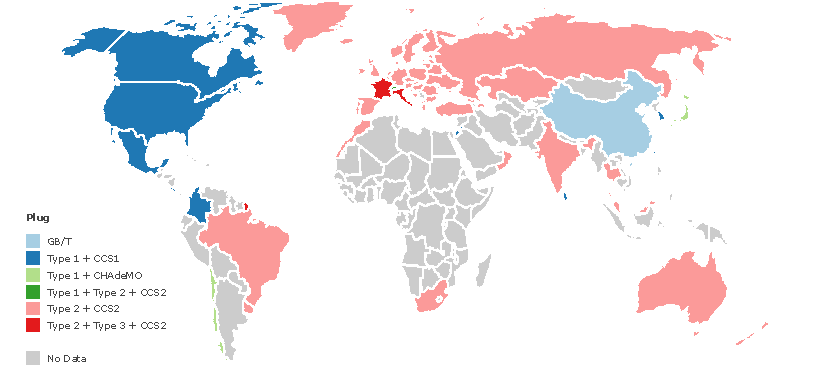
\includegraphics[width=\linewidth]{map}
	\caption[Global EV charging inlet adoption]{Global EV charging inlet adoption~\cite{plugshare_plugshare_nodate}.}
	\label{fig:10:map}
\end{figure}

Fig.~\ref{fig:10:map} shows each country’s predominant AC charging standard in combination with the adopted DC standard. The information used to generate this chart was extracted from the publicly available PlugShare website~\cite{plugshare_plugshare_nodate}, which claims to be the most accurate source of charging stations worldwide, with approximately 112,000 locations and more than 170,000 outlets. Countries that have insufficient or no charging station data are not labelled. 

There are several charging standards omitted from this graph, perhaps most importantly the Tesla charging stations, which provide brand-specific chargers in all countries where they distribute their vehicles. In Australia, China and Pakistan, Tesla DC charging stations outnumber all other DC stations, as shown later in Fig.~\ref{fig:10:worldplug}. When only considering the Type-1, 2 and 3 connectors, Tesla stations outnumber all others in Serbia and Hong Kong.

Charging stations in Western Australia are progressing towards Type-2 chargers. This is inherently visible in recent installations of charging stations, as well as the local charging station networks as follows:

\begin{description}
	\item[] The REV/UWA fast-DC station supports:
	\begin{itemize}
		\item DC CCS Combo Type-2
		\item DC CHAdeMO
	\end{itemize}
	\item[]	while, the RAC stations provide:
	\begin{itemize}
		\item DC CCS Combo Type-1
		\item DC CHAdeMO
		\item AC Type-2 (Mennekes)~\cite{noauthor_ieee_2016}
	\end{itemize}
\end{description}

This variety of outlets allows the stations to support the different EV standards currently in use. All RAC DC-stations have a Level-2 AC station next to them, allowing vehicles without fast-charging support to charge using an SAE J1772 (Type-1) connector. The power and voltage outputs for charging stations that are commonly found around southwest WA is tabulated as Table~\ref{tbl:10:op}.

\nomenclature[z-rac]{RAC}{Royal Automobile Club of Western Australia}

\begin{table}[H]
	\centering
	\caption{Outputs of various charging stations in southwest WA}
	\label{tbl:10:op}
	\begin{tabular}{ccll}
		\toprule
		Type & Phase & Output & Value \\
		\midrule
		\multirow{3}{*}{DC} & \multirow{3}{*}{n/a} & Max output current   & 120 A\\
		& & Max output power     & 50 kW          \\
		& & Output voltage range & 50 -- 500 V DC \\
		\midrule
		\multirow{3}{*}{AC} & \multirow{3}{*}{3} & Max output current   & 63 A     \\
		& & 	Max output power     & 543 kW   \\
		& &			Output voltage range & 400 V AC \\
		\midrule
		\multirow{3}{*}{AC} & \multirow{3}{*}{1} & Max output current   & 32 A     \\
		& &			Max output power     & 7.2 kW   \\
		& &			Output voltage range & 230 V AC ($\pm 10\%$)\\
		\bottomrule
	\end{tabular}
\end{table}

\section{Types of EV Charging}
\label{sec:10:evcharging}
There are several different methods of EV charging. When discussing the efficiency of the various methods this paper does not including any transmission losses or power generation. Various power generation methods for electric vehicle charging can be found here~\cite{speidel_leaving_2016, dell_towards_2014}, with an in-depth comparative study in~\cite{martinez-lao_electric_2017}.  

Electric vehicles are traditionally charged off AC mains. The AC power needs to be converted into DC power by a rectifier inside the vehicle. Although this makes the charging infrastructure quite simple, each EV must carry an expensive and heavy AC-to-DC converter element. In many cases, first generation EVs are equipped with only a basic AC charger, useful for Level-1 home charging (up to 2.4 kW), but not taking advantage of the higher AC currents available at Level-2 charging stations.

The higher the output power of a charger, the heavier and larger the charger must be. Electric vehicles carry this internal charger as a part of their design, to allow charging off a standard electric power point. But at higher currents this method becomes impractical, as larger and heavier AC–DC converters would have to be carried. 

DC stations offer a solution for this. Very little electronics is required in the EV itself, as most of the hardware is included in the charging station. First, EV and station negotiate the correct DC voltage level over a communication link. Then the station provides the correct DC level at a much higher current than is feasible with AC charging. The communication protocol used between the charging station and the vehicle is defined by IEC 61851-1~\cite{international_electrotechnical_commission_iec_2017}.

Signal data lines are part of all charging stations, whether AC or DC, and are fully defined in IEC 62196 and IEC 61851. They are also part of safe-guarding stations and EVs against failures and potential hazards. The stations used in the UWA EV trials were equipped with internal over-voltage/over-current protection, over-heating control, and protective earth detection. The stations were also installed on separate circuits with dedicated RCDs, following the conventions of AS/NZS 3000 Wiring Rules~\cite{standards_association_of_australia_electrical_2018}.

\subsection{Typical Charging Cycle}
Electric vehicles go through three or more different states when charging. This can vary from vehicle to vehicle. At a DC charging system, a battery is typically filled up to only 80\% capacity, as the charging rate significantly slows down for the remaining 20\%, due to the battery’s increase in internal resistance~\cite{tritium_pty_ltd_veefil--electric_2015}.

At most AC charging systems, an EV is fully charged to 100\%, but even then, it continues to draw a small amount of power to maintain the charge of the battery at the top level. This is to counteract the parasitic draw of various electrical systems in the vehicle, and keep the battery full. Some EVs also condition the battery pack through heating or air conditioning, in order to increase charging efficiency~\cite{wang_critical_2016, bullis_electric_2013} or simply pre-condition the cabin through heating or cooling as a comfort feature for the driver. 

Fig.~\ref{fig:10:cr} shows an EV charged from about 25\% to 100\% state of charge (SoC) on the DC charging station at UWA. Although this station can provide 50 kW of power to the EV, charging begins at 40 kW, and as the battery level rises the output power is further reduced. For this reason, all DC charging stations stop charging at 80\% SoC. The remaining 20\% of charging can take longer than the initial 80\% and would preclude other customers from using the charging station.

\begin{figure}[H]
	\centering
	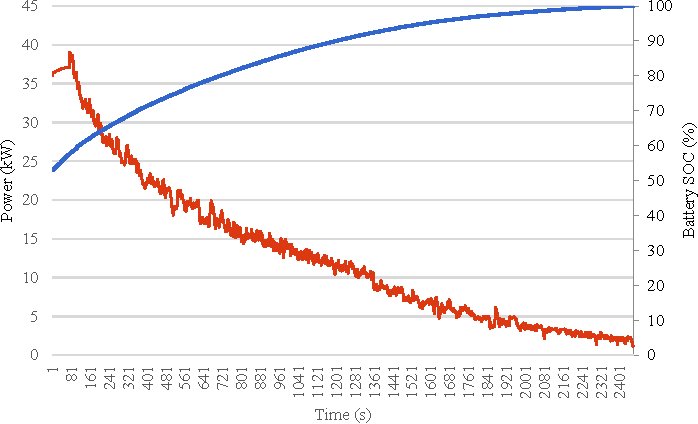
\includegraphics[width=0.7\linewidth]{chargerate}
	\caption[Battery charge rate and State of Charge over time.]{Battery charge rate (kW) in red and State of Charge (\%) in blue over time.}
	\label{fig:10:cr}
\end{figure}

\subsection{Limitations on Charging Speed}
The following factors limit the effective charging speed (or charging power) of a charging station:
\begin{itemize}
	\item \textbf{Temperature of batteries} --- Very high, as well as very low temperatures, require lower charging rates.
	\item \textbf{Temperature of tolerable heat dissipation in the power electronics} --- Examples include charging in closed environments, such as a domestic garage has to limit heat dissipation in order to reduce any fire hazard.
	\item \textbf{Health of the battery} --- Ageing or unhealthy batteries exhibit a larger variation in individual cell voltages and will therefore require more time for balancing during the charging process.
\end{itemize}

\subsection{Authentication and Billing}
Charging station operators may want to control access by some form of user authentication and bill users for their power usage. Authentication can take place in several different ways, including locally at the station (allowing for the station to control authentication without needing an internet connection), or via a server. The charging stations in the REV/UWA trials use RFID cards that were provided to station users. These can be authenticated against an external server. A local whitelist is useful in the event that the station loses its network connection. 

Interfaces to manage these stations are also necessary to collate and display the data to users or operators. The Open Charge Point Protocol (OCPP) was developed in an attempt to foster global development, adoption and compliance of communication protocols~\cite{open_charge_alliance_ocpp_nodate}. This common protocol means that stations from different manufacturers can be controlled by a single OCPP server. 

\subsection{Driving Efficiency and Battery Size for EV}
There is a significant variation in energy efficiency for EVs~\cite{australian_government_green_nodate}, ranging between:
\begin{itemize}
	\item BMW i3: 129 Wh/km
	\item Mitsubishi i-MiEV: 135 Wh/km
	\item Nissan Leaf: 173 Wh/km
	\item Tesla Model S: 186 Wh/km
\end{itemize}
Also, each of these vehicles has a different battery capacity, ranging from the Leaf’s 16 kWh battery to the Tesla Model S 100 kWh battery. For the sake of comparing the different charging stations, two typical scenarios are taken, representing both ends of the spectrum:
\begin{itemize}
	\item Case 1: 16 kWh, 135 Wh/km
	\item Case 2: 100 kWh, 200 Wh/km
\end{itemize}

\subsection{Inductive Charging}
Inductive charging allows wireless charging of an EV via an electromagnetic field.  There is a coil in the vehicle and one located below the vehicle, usually embedded in a mat. Of the various charging methods, this is the least efficient but the most convenient, as it does not require the driver to plug the vehicle or even to carry a cable. A major issue that manufacturers need to address is that the efficiency is reduced if the coils are not aligned correctly when parked. Only 5\% of the surveyed EVs parked within the tolerance level of the coils, so this requires either a movable coil or a self-parking vehicle to reduce this issue~\cite{birrell_how_2015}. The power transfer efficiency varies depending on the manufacturer, air gap and power rating. In seven different studies between 2011 and 2014 these values were found to be between 83\% and 92\%~\cite{kalwar_inductively_2015}. 

\subsection{Level-1 Charging (IEC 62196-3 Mode 2)}
Level-1 is limited by the rating of a standard power outlet in the respective country. In Australia, the maximum power to be drawn at Level-1 is 240 V at 10 A (2.4 kW). Electric vehicles are mostly fitted with these chargers internally, as they are comparatively lightweight.

\subsection{Level-2 Charging (IEC 61851-3 Mode 3)}
Level-2 charging allows the vehicle to draw a higher current up to 32 A at 240 V (7.7 kW for single phase or 23 kW for three phase). Like Level-1 charging, this relies on the internal charger of the vehicle.

\subsection{DC-Fast Charging (IEC 61851-3 Mode 4)}
DC-fast charging ranges from 50–-900 V DC and has a range of varying current outputs. Unlike other stations, the charger is not inside the vehicle, but within the station itself. The station’s charger is controlled by the vehicle via data lines. The stations in WA support up to 125 A (50 kW), while Tesla's Supercharger already charges at 120 kW~\cite{tesla_supercharger_nodate}. Recent CCS 2.0 stations are supplying up to 350 kW per station~\cite{charging_interface_initiative_e._v._ccs_2018}, while future CCS DC chargers will deliver up to 450 kW per station~\cite{lambert_bmw_2017, kane_fastcharge_2017}.

\subsection{Alternate Methods}
Another potential method of converting AC power into DC for charging the vehicle is through the use of integrated motor drives where the vehicles’ motors are used to do the conversion~\cite{johansen_fast-charging_2013}. 

\subsection{Charging Speed Comparison}
Table~\ref{tbl:10:techniques} compares the various charging techniques for different battery types and charging levels.
\begin{table}[H]
	\centering
	\caption{Charging style configuration and time for small and large battery packs}
	\label{tbl:10:techniques}
	\begin{tabular}{lcrr}
		\toprule
		\multirow{2}{*}{Charging Type} & \multirow{2}{*}{Charge level} & \multicolumn{2}{c}{Charging time} \\
		\cmidrule(l){3-4}              &                               &   16 kWh    &       100 kWh       \\ \midrule
		Level-1                        &             100\%             &   5 hours   &      33 hours       \\
		Level-2 (1-phase)              &             100\%             &   2 hours   &      11 hours       \\
		Level-2 (3-phase)              &             100\%             & 40 minutes  &      3.7 hours      \\
		DC   50 kW                      &             80\%              & 15 minutes  &      1.5 hours      \\
		DC 150 kW                       &             80\%              &  5 minutes  &     32 minutes      \\
		DC 450 kW                       &             80\%              & 1.7 minutes &    10.7 minutes     \\ \bottomrule
	\end{tabular}
\end{table}

\subsection{Australian Charging Standard Preference}
Fig.~\ref{fig:10:ausplug} presents a chart of the number of charging stations installed in Australia. In total 416 stations have been registered at online platform PlugShare.

\begin{figure}[H]
	\centering
	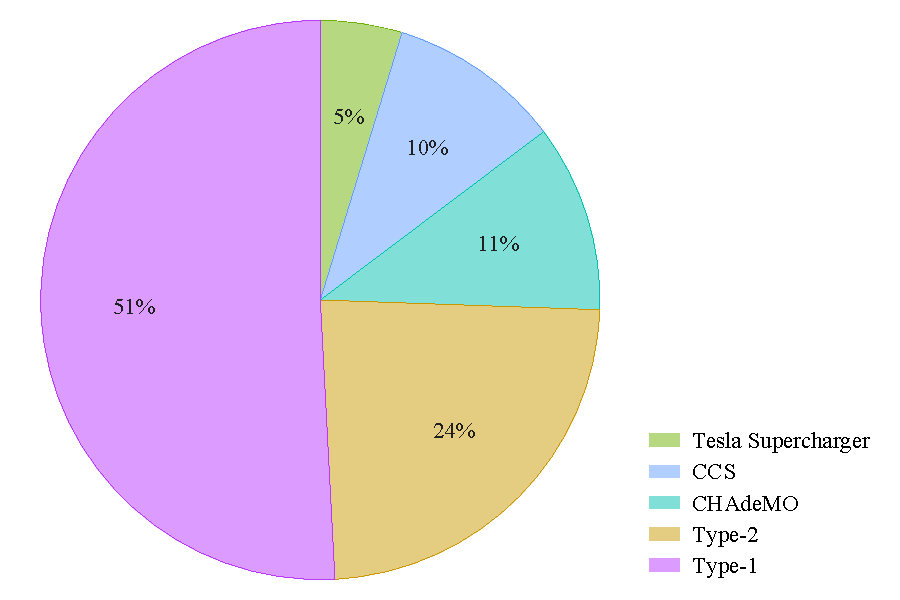
\includegraphics[width=0.7\linewidth]{ausplug}
	\caption{Australian charging inlet adoption.}
	\label{fig:10:ausplug}
\end{figure}

It was observed that there are slightly more installations for CHAdeMO than CCS in Australia, but CCS is expected to take over within two years, as there is a shift to more CCS inlets from major car manufacturers.
BMW as one of the market leaders, has decided to swap over from Type-1 to Type-2 EV inlets for the Australian market and it is expected that will trigger other OEMs to follow suit. Standards Australia has so far failed to recommend any charging standard although the topic has been debated for over ten years. Out of the 416 stations registered, there are:
\begin{itemize}
	\item 20 Tesla Superchargers,
	\item 41 CCS,
	\item 45 CHAdeMO,
	\item 98 Type-2, and
	\item 212 Type-1 stations. 
\end{itemize}

\subsection{International EV Plug Adoption}
The global adoption of DC charging inlets from about 147,911 charging stations worldwide was also analysed, as illustrated in Fig.~\ref{fig:10:worldplug}.

\begin{figure}[H]
	\centering
	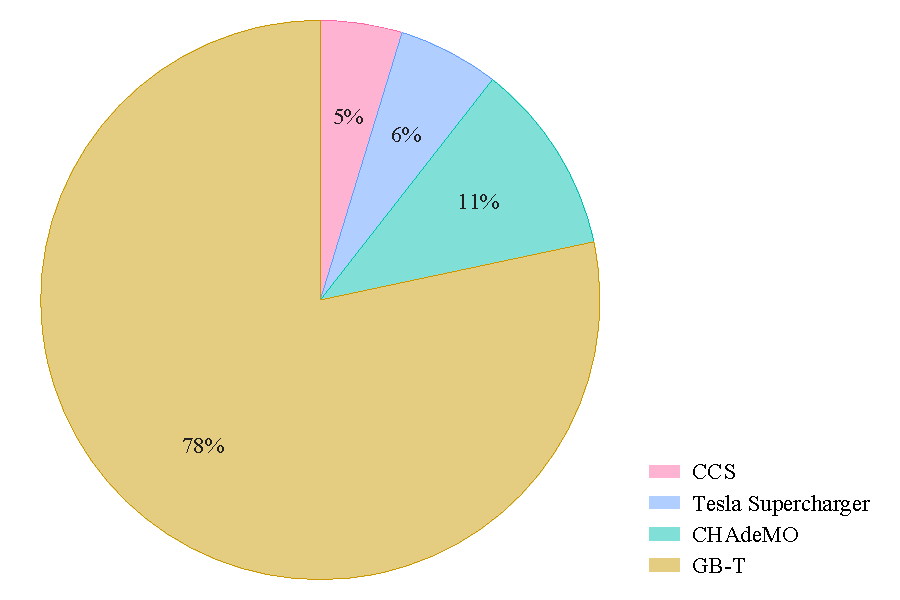
\includegraphics[width=0.7\linewidth]{worldplug}
	\caption{Global DC charging inlet adoption.}
	\label{fig:10:worldplug}
\end{figure}
 
The Chinese GB/T standard has the highest share of all worldwide charging installations, but only exists in China, due to the Chinese government’s New Energy Vehicle (NEV) initiatives in 2009, which catalysed the installations of charging stations around the country~\cite{ji_plug-electric_2018}. CHAdeMO, originating in Japan, was introduced prior to CCS and has many installations in Japan and North America, leading to its higher market share. Of the charging stations in Figure 4, there are:
\begin{itemize}
	\item 115,776 GB/T DC chargers, of which 66,059 are combined AC/DC stations~\cite{china_electric_vehicle_charging_infrastructure_promotion_alliance_zhongguo_2017}
	\item 16,639 CHAdeMO stations,
	\item 8,496 Tesla Superchargers, and
	\item 7,000 CCS stations~\cite{steitz_plug_2018}.
\end{itemize}

\nomenclature[z-nev]{NEV}{New energy vehicle}

\section{Analysis of Charging Station Usage}
\label{sec:10:analysis}
Usage patterns of the UWA/REV charging station network were analysed, comprising 20 7 kW AC chargers and a 50 kW DC-fast charger. Data was obtained during the period of 1 June 2012 through 31 January 2018 for the AC stations, and from 12 November 2014 through 13 October 2017 for the DC station, unless stated otherwise. Short dates are presented in the format ``dd/mm/yyyy''.

\subsection{AC Charging and Maintaining Charge}
\label{sec:10:ac}
UWA/REV stations are Level-2 stations which typically require a few hours to fully charge a vehicle and therefore many users leave their vehicles charging while they are at work. Many vehicles are hence idly plugged into the charging station even when charging has been completed. Of course, this is mostly because no fees are being collected for charging or for parking at these stations. In this section the charging patterns of the UWA AC stations were analysed across the data summary tabulated in Table~\ref{tbl:10:acstats}. To ensure that only real charging events are logged, events that are less than five minutes long are filtered.

\begin{table}[H]
	\centering
	\caption{Total statistics for the AC stations across the sample period}
	\label{tbl:10:acstats}
	\begin{tabular}{ll}
		\toprule
		Number of events & 4,444 \\
		Total energy delivered & 29,206 kWh \\
		Total plugged in time & 672 days \\
		\bottomrule
	\end{tabular}
\end{table}

\begin{figure}[H]
	\centering
	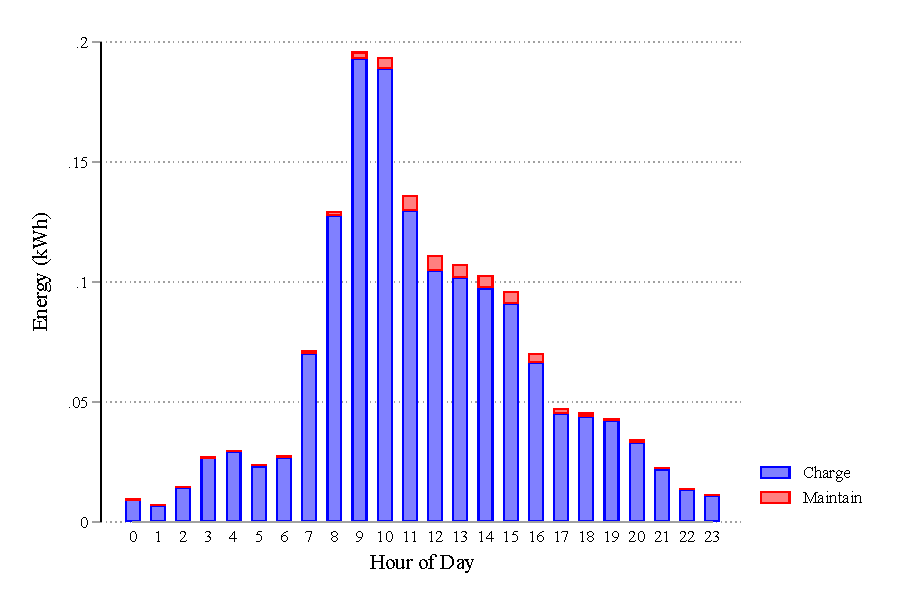
\includegraphics[width=0.8\linewidth]{ac_h_e}
	\caption[Energy delivered for an AC station at each hour of day]{The energy delivered during charging and maintaining charge on average for an AC station at each hour of day.}
	\label{fig:10:ac_h_e}
\end{figure}

Fig.~\ref{fig:10:ac_h_e} illustrates the average energy delivery of an AC charging station at each hour of day. Energy delivery increases and peaks at 9 am because it is then when many users arrive at work to charge their vehicle. The energy used to maintain charge increases and peaks at 12 noon, when most of the vehicles have been fully charged. That said, the average energy used to maintain charge on a vehicle averages at only 2.19 Wh, which is significantly below the average charging energy of 63.3 Wh.

\begin{figure}[H]
	\centering
	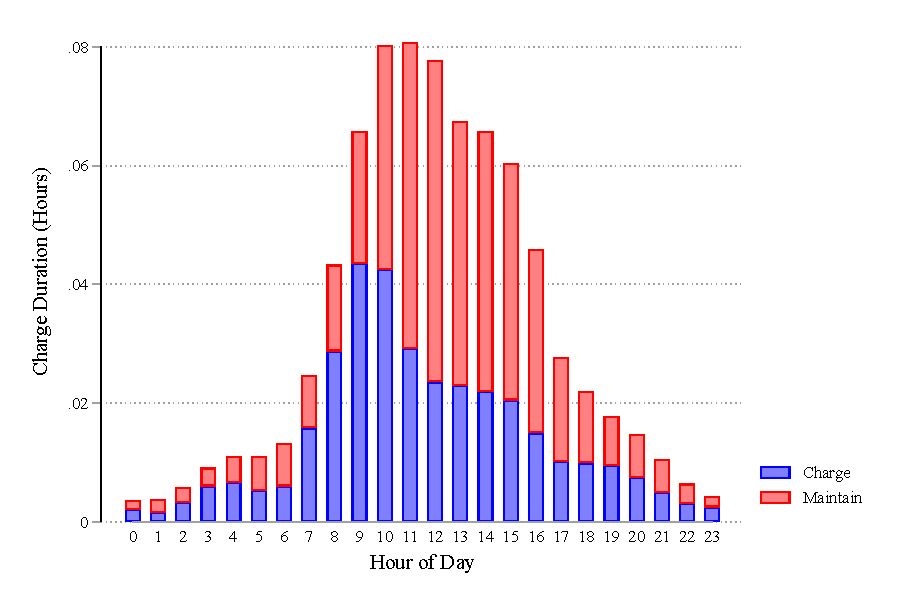
\includegraphics[width=0.8\linewidth]{ac_h_c}
	\caption[Durations of AC charge per station at each hour of day]{Durations of charging and maintaining AC charge by station time on a vehicle per station at each hour of day.}
	\label{fig:10:ac_h_c}
\end{figure}


Fig.~\ref{fig:10:ac_h_c} shows the average time spent for an AC charging station to be in charging or maintaining state over the time of day. As most charging events commence around 9 am to 10 am, more time is spent charging at the station, and as the vehicles get charged, the ``charge bar'' in the graph eventually transitions into the ``maintain bar'' for the rest of the vehicle's plug-in time. The charging stations free up in the evenings, before demand increases again in the next morning. In total, the UWA/REV AC stations have spent 312 days charging and 405 days maintaining charge over the data collection time frame, which averages to 0.342 hours charging and 0.431 hours maintaining per day per station. The average charge event at an AC station takes 3.91 hours and uses 6.66 kWh of energy.

\begin{figure}[H]
	\centering
	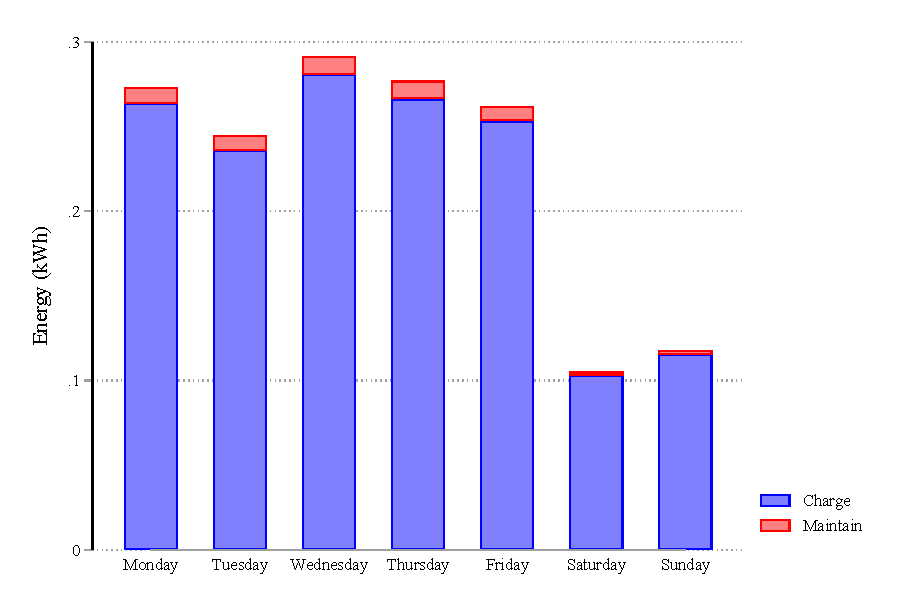
\includegraphics[width=0.8\linewidth]{ac_d_e}
	\caption[Energy delivered for an AC station for each day of week]{The energy delivered during charging and maintaining charge on average for an AC station for each day of week.}
	\label{fig:10:ac_d_e}
\end{figure}

By analysing the charging patterns across a week, Fig.~\ref{fig:10:ac_d_e} indicates that more energy is used during the weekdays for charging, at an average of 0.27 kWh per day. Charger usage drops significantly on weekends to less than half at 0.11 kWh per day. 

\begin{figure}[H]
	\centering
	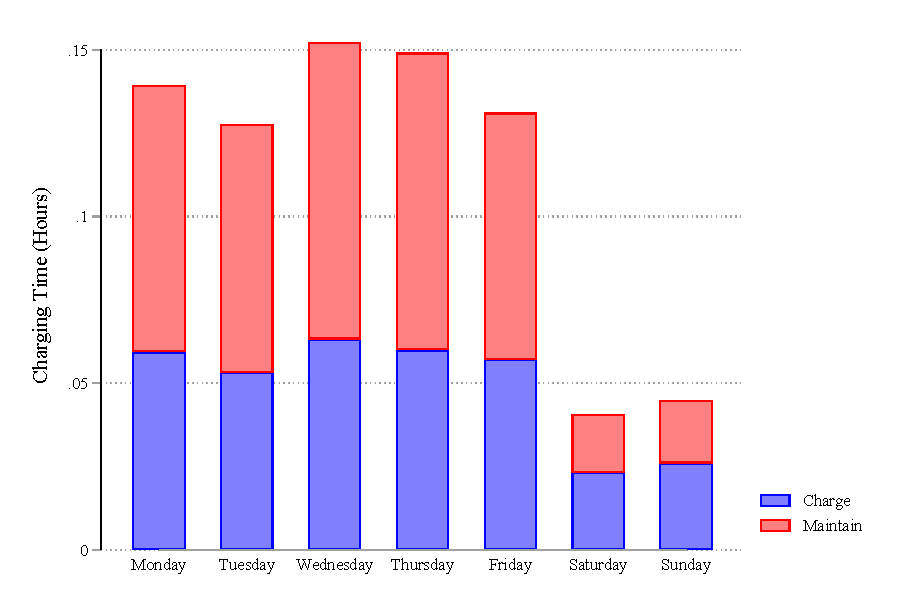
\includegraphics[width=0.8\linewidth]{ac_d_h}
	\caption[Time taken to AC charge a vehicle for each day of week]{The time taken to charge or maintaining AC charge on a vehicle for each day of week. (CS vs DC).}
	\label{fig:10:ac_d_h}
\end{figure}


When comparing charge times across the days of the week, Fig.~\ref{fig:10:ac_d_h} shows that charging duration decreases during the weekends by 53\% on average, each station spends 0.14 hours charging and maintaining on weekdays, and 0.043 hours on weekends. This is consistent with the results from Fig.~\ref{fig:10:ac_d_e}.

\begin{figure}[H]
	\centering
	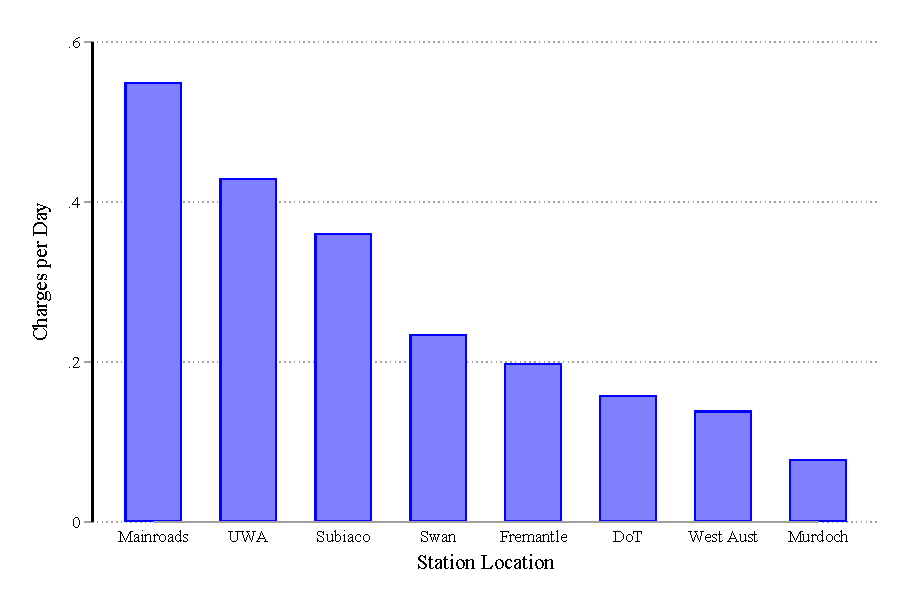
\includegraphics[width=0.8\linewidth]{ac_p_c}
	\caption[Number of chargers per day between each AC station]{Comparison for the number of chargers per day between each of the AC stations.}
	\label{fig:10:ac_p_c}
\end{figure}

A comparison of the average daily number of charge events for each UWA/REV AC charging station is shown in Fig.~\ref{fig:10:ac_p_c}. The low number of charges per day is mostly due to slower charging on AC and the fact that cars are not collected when charging is finished, so charging bays are not freed up for new customers. The charger locations near offices and work locations enable their staff to charge on a more consistent basis, but it leaves the stations vacant on weekends. This is evident in the UWA Computer Science and Main Roads stations, where staff charge their vehicles daily on weekdays. The stations in the suburbs of Subiaco and Fremantle are in general parking areas and are more accessible to the public. However, the low EV penetration rate combined with the long charging times contributes to lower charging numbers for these stations. Overall, UWA/REV AC stations have on average 0.27 charges per day, ranging from 0.08 to 0.55 charges per day.

\begin{figure}[H]
	\centering
	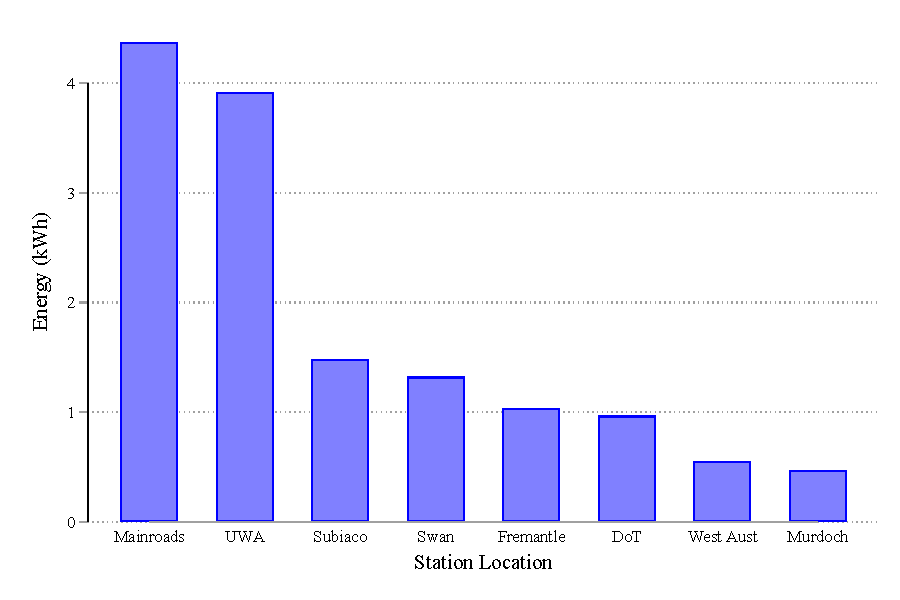
\includegraphics[width=0.8\linewidth]{ac_p_e}
	\caption[Energy delivered at each AC station per day]{Comparison for the energy delivered at each station per day across each of the AC stations.}
	\label{fig:10:ac_p_e}
\end{figure}

By comparing the energy delivery per day for each AC station, Fig.~\ref{fig:10:ac_p_e} shows a similar trend to Fig.~\ref{fig:10:ac_p_c}, whereby a higher charge per day will contribute to a higher energy usage for each station. Each station delivers on average 1.76 kWh per day, with the Main Roads station delivering the most energy at 4.38 kWh per day.

\subsection{AC versus DC Station Comparison (CS vs DC)}
A comparison of the UWA/REV fast-DC station against the AC station network at the UWA Computer Science (CS) car park is shown in Fig.~\ref{fig:10:acdc_e}. As expected, the DC station delivers much higher energy amounts in a shorter time than the AC station. 

\begin{figure}[H]
	\centering
	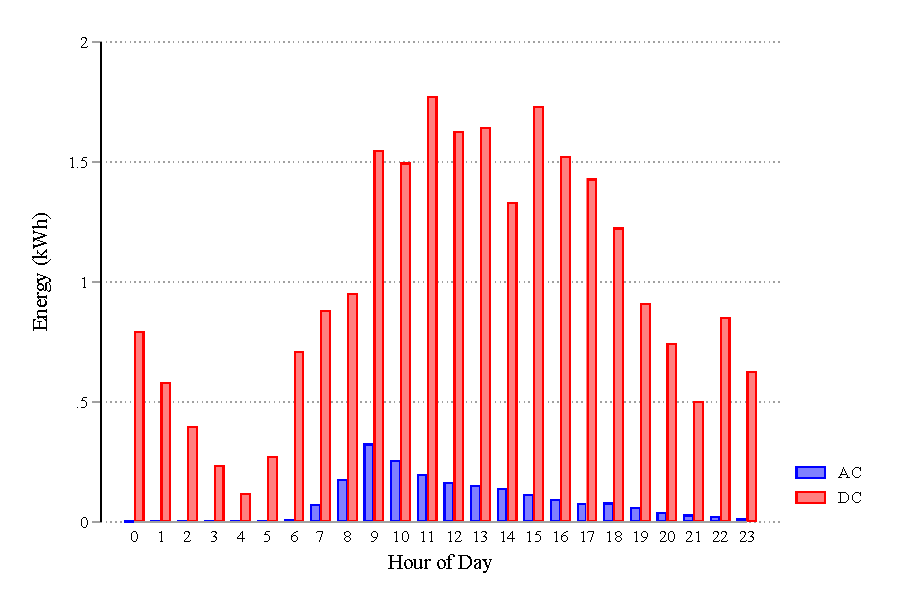
\includegraphics[width=0.8\linewidth]{acdc_e}
	\caption[Energy delivered by an AC station versus a DC station]{The differences in energy delivered by an AC station versus a DC station at each hour of day (CS vs DC).}
	\label{fig:10:acdc_e}
\end{figure}

Fig.~\ref{fig:10:acdc_e} compares the energy usage between the DC station and the AC station across each hour of day based on its charge events. The energy used for the AC station is the sum of its energy delivery during charging and maintaining phases. The DC station uses 7.78 times more energy per hour than the AC station. On average, the AC station delivers 0.09 kWh per hour, while the DC station delivers 1.0 kWh per hour. Also, while the energy delivery at the AC station peaks at 9 am, charging events at the DC station usually peak later in the morning and continue into the afternoon and evening. The quick charging capability of the DC stations means that users can often charge their vehicle en route to their destination. 

\begin{figure}[H]
	\centering
	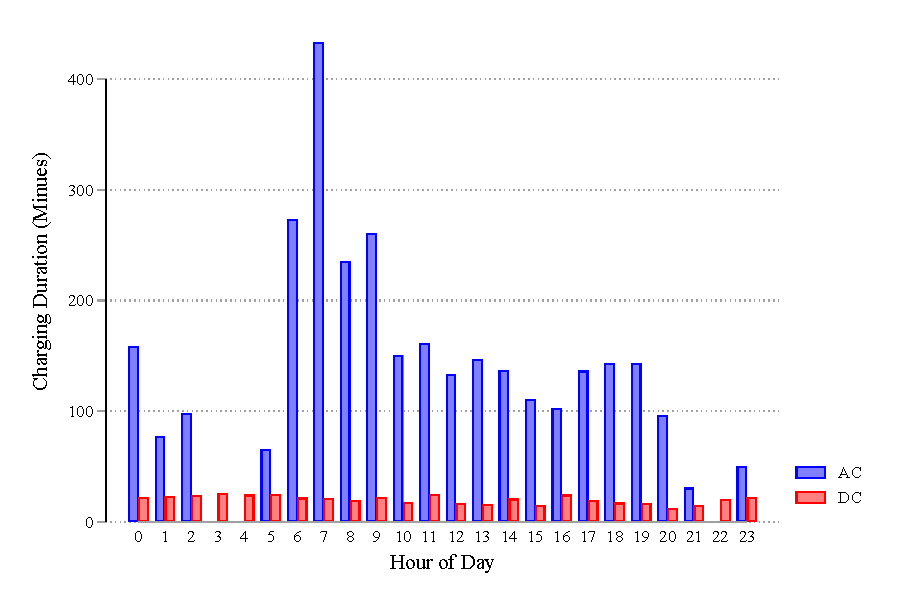
\includegraphics[width=0.8\linewidth]{acdc_h}
	\caption[Charging time on an AC station versus a DC station]{The difference in charging time on an AC station versus a DC station at each hour of day.}
	\label{fig:10:acdc_h}
\end{figure}

Fig.~\ref{fig:10:acdc_h} compares the charging duration between the UWA DC station and the UWA AC station per hour of day. Charging durations for the AC station is a sum of its charging and maintaining phases. On average, vehicles are tethered to an AC station 6.5 times longer than at a DC station. Even so, there is only a 13.3\% difference in the energy delivered between the DC and AC charge events. 

It is noted that while charging durations on the AC station are longest for morning arrivals, there is no such noticeable trend for DC charging durations. 

\begin{figure}[H]
	\centering
	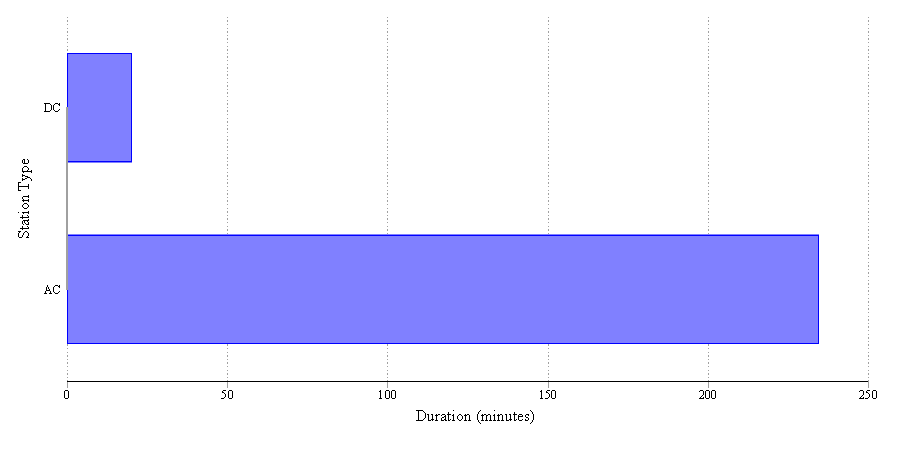
\includegraphics[width=0.8\linewidth]{acdc_t_h}
	\caption{The average charging duration for a DC and AC charge event.}
	\label{fig:10:acdc_t_h}
\end{figure}

Fig.~\ref{fig:10:acdc_t_h} compares the average charging duration for each charge event on the REV/UWA DC and AC stations. The data for AC charging is averaged across all charging events on all AC stations. The average AC charging time across all metropolitan stations is 235 minutes (3h55min) for 6.65 kWh, while the average DC charging takes 20.2 minutes for 7.80 kWh.

\begin{figure}[H]
	\centering
	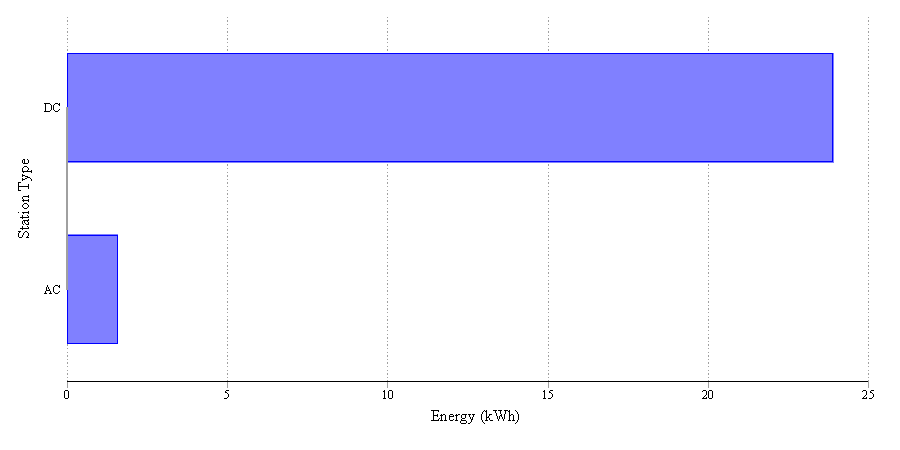
\includegraphics[width=0.8\linewidth]{acdc_t_e}
	\caption{The daily energy delivery for a DC and AC station.}
	\label{fig:10:acdc_t_e}
\end{figure}

When comparing the daily energy delivery between the AC and DC charging stations, Fig.~\ref{fig:10:acdc_t_e} illustrates that the DC station typically delivers 23.9 kWh per day, and 1.57 kWh per day for an AC station.

\subsection{DC Station Comparison}
\label{sec:10:dc}
Comparing data from the UWA DC station with the Electric Highway DC stations in the WA South-West, the number of charge events, charging duration and the energy delivered is considered.

\begin{figure}[H]
	\centering
	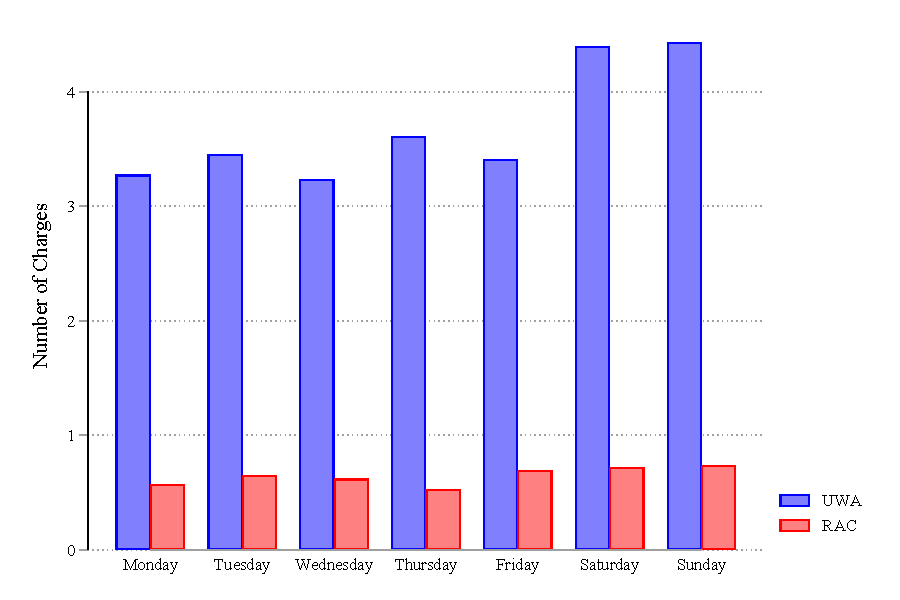
\includegraphics[width=0.8\linewidth]{uwarac_c}
	\caption[Number of DC charge events per station per day of week]{Number of DC charge events per station per day of week between the UWA (12/11/2014 to 13/10/2017) and the Electric Highway (RAC) (02/03/2016 to 20/09/2016).}
	\label{fig:10:uwarac_c}
\end{figure}

The number of charges per day of week in Fig.~\ref{fig:10:uwarac_c} compares the average charges at UWA with the RAC stations. The charging data from the RAC stations is compared with the UWA/REV data across 2,370 recorded charging instances beginning from 12 November 2014 to 13 October 2017. The average number of DC charge events is 3.35 per day at UWA, but only 0.65 per day for the average Electric Highway station. 

\begin{figure}[H]
	\centering
	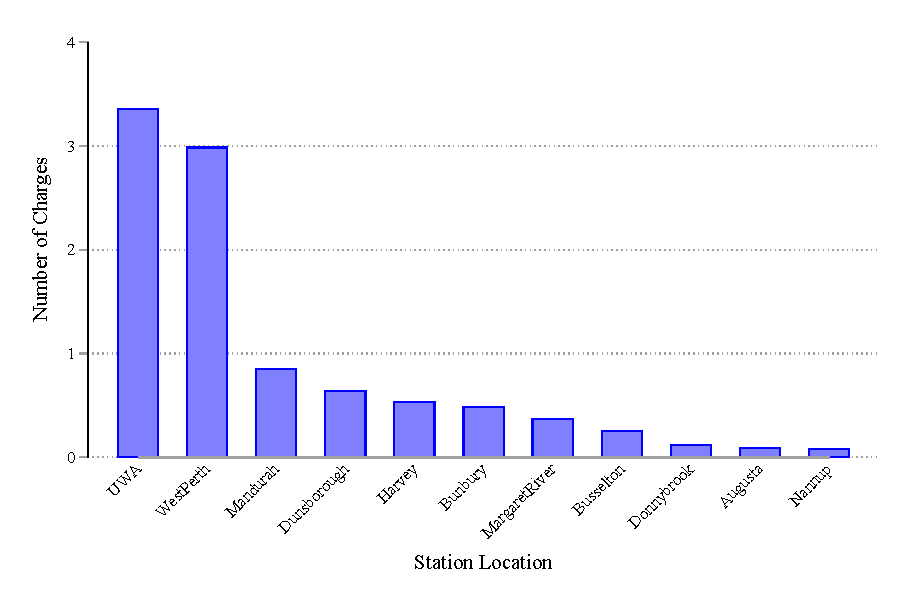
\includegraphics[width=0.8\linewidth]{dc_p}
	\caption[Number of charges per day for each station]{The number of charges per day for each station from the UWA (12/11/2014 to 13/10/2017) and the RAC (02/03/2016 to 20/09/2016).}
	\label{fig:10:dc_p}
\end{figure}

By comparing the number of charges per day for each station, Fig.~\ref{fig:10:dc_p} shows that the stations closer to the Perth CBD are used more often than those in regional areas. The RAC West Perth station has 3.0 charges per day, whereas the UWA station has 3.35 charges per day. The regional stations have significantly fewer than 1.0 charge per day, with Mandurah at 0.86 charges per day, and the lowest being Nannup at 0.087 charge events per day. This puts the average number of charge events of an Electric Highway station to 0.65 charges per day.

\nomenclature[z-cbd]{CBD}{Central business district}
\nomenclature[z-cs]{CS}{Computer science}

\begin{figure}[H]
	\centering
	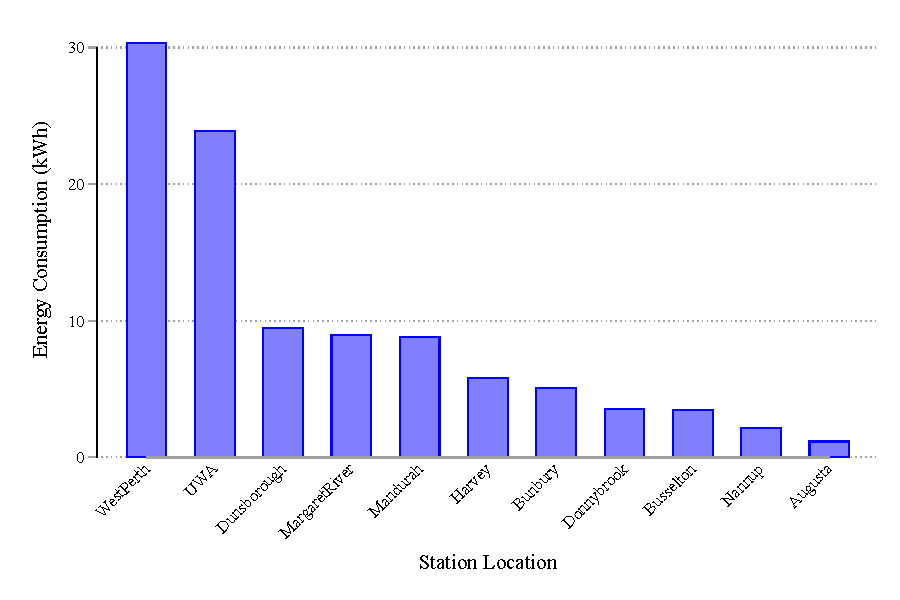
\includegraphics[width=0.8\linewidth]{dc_p_e}
	\caption[Amount of energy delivered per day for each station]{The amount of energy in kWh delivered per day for each DC station from the UWA (12/11/2014 to 13/10/2017) and the RAC (02/03/2016 to 20/09/2016).}
	\label{fig:10:dc_p_e}
\end{figure}

Energy delivery across all stations per day is in line with their number of charge events in Fig.~\ref{fig:10:dc_p}, whereby stations in the city deliver more energy per day. However, despite their lower charging frequency, regional stations deliver more energy per charge as illustrated in Fig.~\ref{fig:10:dc_p_e}. The West Perth station delivers the most energy at 30.4 kWh per day, followed by the UWA station at 23.9 kWh. The Augusta station delivers the least amount of energy at 1.2 kWh per day. The average energy delivered by the Electric Highway stations comes to 7.92 kWh per day.

\begin{figure}[H]
	\centering
	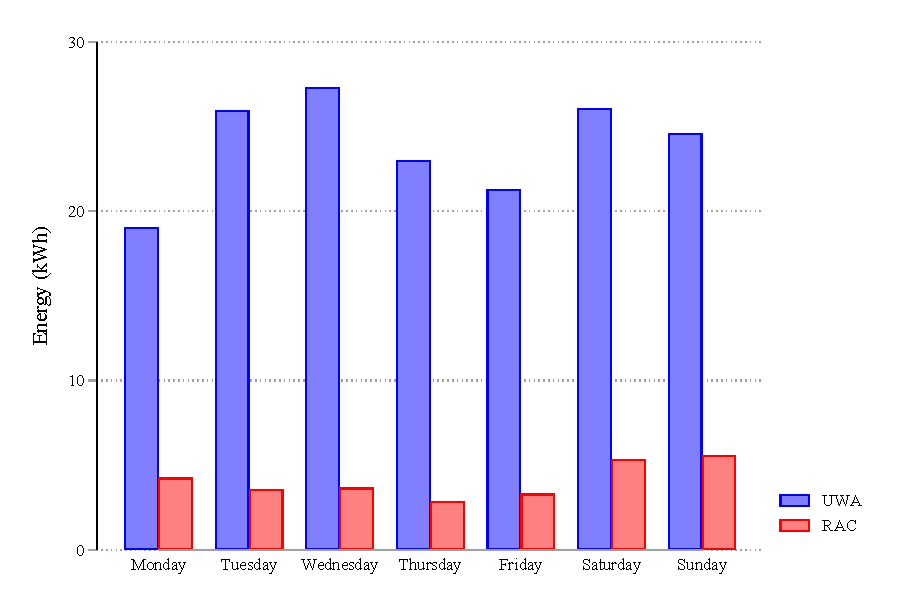
\includegraphics[width=0.8\linewidth]{uwarac_e}
	\caption[Energy delivered per station per day of week]{The energy delivered per station per day of week between the UWA (12/11/2014 to 13/10/2017) and the Electric Highway (RAC) (02/03/2016 to 20/09/2016) DC stations.}
	\label{fig:10:uwarac_e}
\end{figure}

Fig.~\ref{fig:10:uwarac_e} compares the energy usage between the UWA station and the average Electric Highway station across each day of the week. The Highway stations are more popular during weekends, as more traffic commutes to regional destinations. On average the Highway stations consume 5.55 kWh on a Sunday as compared to 2.88 kWh on a Thursday. The UWA charging station delivers the most energy on Wednesday with 27.3 kWh, and the least on Monday with 19 kWh.

\begin{figure}[H]
	\centering
	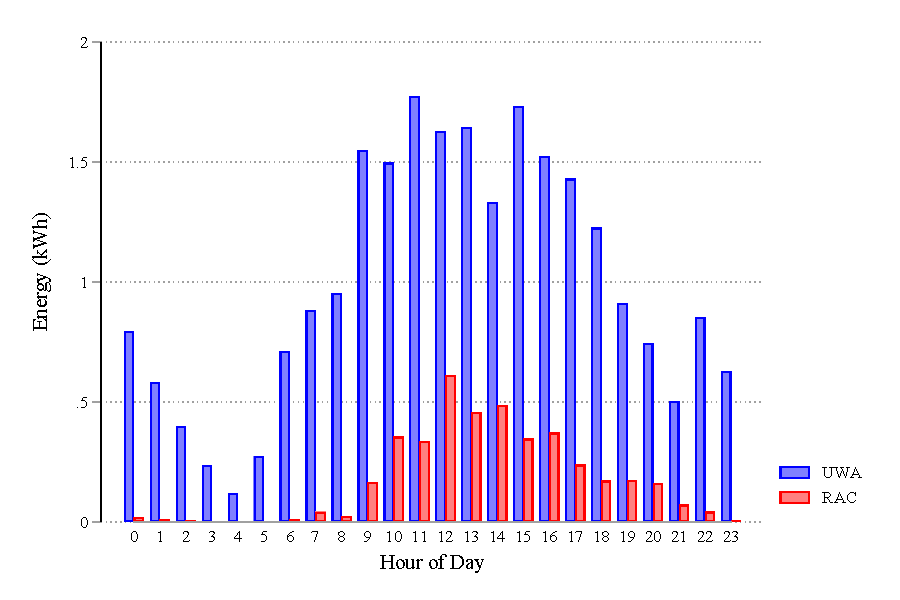
\includegraphics[width=0.8\linewidth]{uwarac_h_e}
	\caption[Energy delivered per station per hour of day]{The energy delivered per station per hour of day between the UWA (12/11/2014 to 13/10/2017) and the RAC (02/03/2016 to 20/09/2016) DC stations.}
	\label{fig:10:uwarac_h_e}
\end{figure}

Fig.~\ref{fig:10:uwarac_h_e} compares the energy consumption per time of day between the UWA station and the average of the RAC charging stations. This data was averaged through all the historical charges on the UWA station, which was then classified to its instantaneous energy consumption at each hourly duration per day. This data is then compared with the data that was obtained from the RAC stations. On average, the UWA station delivers 23.9 kWh per day, while the average Highway station delivers 4.08 kWh per day. 

\begin{figure}[H]
	\centering
	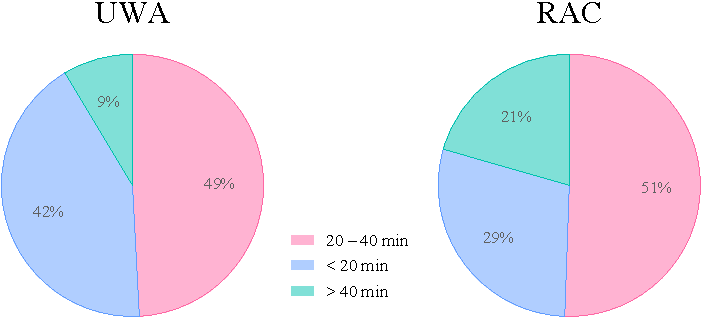
\includegraphics[width=0.8\linewidth]{dur}
	\caption[Average charging durations on the DC stations.]{The average charging durations on the UWA (12/11/2014 to 13/10/2017) and the Electric Highway (02/03/2016 to 20/09/2016) DC stations.}
	\label{fig:10:dur}
\end{figure}

Charging durations at the UWA stations, as shown in Fig.~\ref{fig:10:dur}, are predominantly under 40 minutes, which makes up 89\% of all charges. The average charging time for the UWA DC station is 22.45 minutes. Half of the charges at the Electric Highway stations take between 20 to 40 minutes, with 29\% taking less than 20 minutes. The average charging time for the Electric Highway DC stations is 30.68 minutes.

\begin{table}[H]
	\centering
	\caption[Comparison of average charging duration and energy consumption]{Comparison of average charging duration and energy consumption for AC and DC stations (02/03/2016 to 20/09/2016).}
	\label{tbl:10:acdcdur}
	\begin{tabular}{clrr}
		\toprule
		Type & Owner          & Duration (hh:mm) & Energy (kWh) \\ \midrule
		DC   & UWA            &            00:21 &        7.128 \\
		     & Highway        &            00:31 &        12.26 \\ \midrule
		AC   & UWA (7 kW)     &            05:11 &        9.811 \\
		     & Highway (7 kW) &            02:01 &        4.313 \\
		     & Highway (43kW) &            01:19 &        16.69 \\ \bottomrule
	\end{tabular}
\end{table}

Table~\ref{tbl:10:acdcdur} summarises the average charging duration and energy consumption per charge on AC or DC charging stations of UWA and RAC. Comparing the DC charge times, users of an RAC DC station charge 10 minutes longer on average and delivered 4.6 kWh more energy than they do at the UWA station. This is mostly contributed by the West Perth station, which is more frequented by drivers due to its close proximity to the city centre, which implies that drivers can visit the nearby shopping centre and cafes while their vehicle is charging. Conversely, charging durations are longer at the UWA/REV AC stations (of which half are installed near workplaces) when compared to the RAC 7 kW AC stations, which average to about 1.5 hours longer and 2.83 kWh more energy delivered. The 43 kW fast-AC chargers average at 1.3 hours charge time, delivering 16.69 kWh of energy. The average charging time per vehicle on the UWA DC station is 21 minutes to take, on average, 7.1 kWh of energy. For the Highway stations, the average charging time is 31 minutes for 12.26 kWh of energy.

\subsection{DC Charging Connectors Used}
Fig.~\ref{fig:10:uwaplug} compares the types of connectors used at the UWA DC station. CHAdeMO (88\%) is in higher demand than CCS (12\%) which is because popular EV models from Mitsubishi and Nissan use CHAdeMO, and Tesla provides a CHAdeMO adapter for their vehicles. This trend is set to change with the introduction of more EVs with CCS connectors in Australia from the 2018 model year onwards. 

\begin{figure}[H]
	\centering
	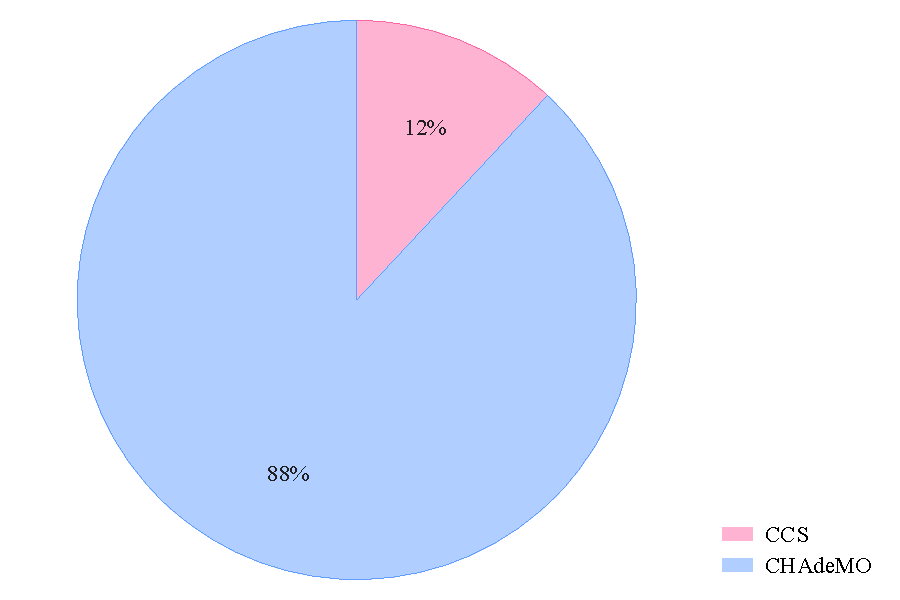
\includegraphics[width=0.7\linewidth]{uwaplug}
	\caption[Percentage of connector types used at the UWA DC station]{Percentage of connector types used at the UWA DC station (12/11/2014 to 13/10/2017).}
	\label{fig:10:uwaplug}
\end{figure}

\section{Cost Modelling}
\label{sec:10:cost}
Table~\ref{tbl:10:cost} introduces a cost model that includes the usage analysis as summarised in Section~\ref{sec:10:analysis}. This is presented as a probabilistic case study for running and maintaining various types of charging stations, namely 7 kW AC (AC-7), 50 kW DC (DC-50), 150 kW DC (DC-150) and 350 kW DC (DC-350).

The stations’ running costs are calculated per day based on the costs associated to their estimated purchasing and installation costs, while assuming a financing option and depreciation of 5\% and 8\% per annum respectively over its lifespan. Energy tariffs are based on ongoing rates from Synergy, which is the sole residential energy provider in metropolitan WA. Based on observations, new stations are expected to be provisioned for ten years before needing replacements or large-scale maintenance. The total running cost includes estimated ongoing maintenance cost, and the option of parking bay rental. Calculations of the sales required to break even include scenarios where bay rental is needed or otherwise. \textit{Actual energy} and charging time values are based on data collection from the UWA/REV stations. The \textit{estimated} use subject illustrates conservative estimates for utilisation of more powerful DC stations under a higher EV adoption rate. 

A station running cost $C_r$ is calculated as the sum of its finance interest, depreciation and its operating/maintenance cost per day, adding its energy supply cost and if applicable, its bay lease.
\begin{align}
C_r = \frac{i + D + C_m}{365.25} + \frac{C_{sup}}{S}[+C_s]
\end{align}  
Using estimates for $i$, $D$, and $C_m$ in Table~\ref{tbl:10:cost}, along $C_{sup}$ provided by Synergy, the running cost for the 7 kW AC, 50 kW DC, 150 kW DC and 350 kW DC stations was calculated to be \$2.11, \$13.81, \$28.99 and \$57.62 respectively, excluding an estimated bay lease of \$10 per day. These figures scale exponentially with the charging station’s power output, as more powerful stations are more expensive and require more energy to operate. This is, however, compensated with faster charging durations, allowing a higher charge frequency.

\nomenclature[a-c]{$C$}{Cost [Chapter~\ref{ch:charging}]}
\nomenclature[a-i]{$i$}{Interest}
\nomenclature[s-m]{$m$}{Operation/maintenance}
\nomenclature[s-sup]{$sup$}{Energy supply}
\nomenclature[s-r]{$r$}{Running}
\nomenclature[a-m]{$M$}{Profit margin [Chapter~\ref{ch:charging}]}
\nomenclature[a-r]{$R$}{Break-even energy sales}
\nomenclature[s-b]{$B$}{Bay lease}
\nomenclature[a-t]{$T$}{Tariff}
\nomenclature[s-e]{$E$}{Energy}
\nomenclature[s-d]{$d$}{Delivery}
\nomenclature[s-c]{$C$}{Charging instance}
\nomenclature[a-n]{$N$}{Number set}
\nomenclature[a-S]{$S$}{Charging station count}
\nomenclature[a-t]{$t$}{Time period}
\nomenclature[s-e]{$L$}{Lifespan}
\nomenclature[s-d]{$D$}{Depreciation}

To calculate the required break-even energy sales $R$ for each charging station to break even, scenarios with profit margins $M$ at 50\% and 100\%, with or without the bay lease of \$10/day ($B$/$\bar{B}$) were considered. The energy tariff $T_E$ is referenced to Synergy, which at time of writing stands at \$0.28327/kWh. 
\begin{align}
R = \frac{C_r}{M \cdot T_E}
\end{align}
The calculated sales requirements $R$ to break-even for these four scenarios across the four charging station types is then plotted as illustrated in Fig.~\ref{fig:10:costm}.

\begin{figure}[H]
	\centering
	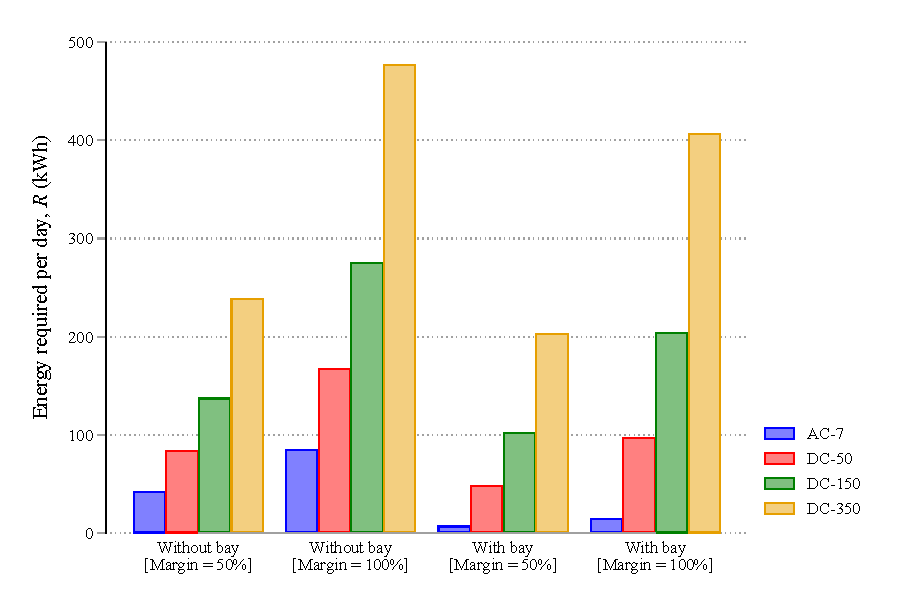
\includegraphics[width=0.8\linewidth]{costm}
	\caption[Break-even points on required energy delivery]{Break-even points for the AC and DC stations' energy delivery in kWh required under scenarios representing with or without bay rentals $C_B$ (Bay/No bay), with sales margins set at 50\% ($M=0.5$) and 100\% ($M=1$).}
	\label{fig:10:costm}
\end{figure}

From Fig.~\ref{fig:10:costm}, it is clear that any fee for the charging bay rental $C_B$ increases the required break-even energy sales requirement $R$, but it has a lower relative effect on the higher-output DC stations, which are expected to sell more energy per day accordingly. For instance, the presence of the bay rental fee $C_B$ across both margins increases the break-even point $R$ by 573\% on the 7 kW AC station, which means this station will never be profitable in this scenario.

For 50 kW, 150 kW and 350 kW DC stations, break-even point R increases to 172\%, 134\% and 117\%, respectively. This results in less impact for faster stations. Increasing the sales margins from 50\% to 100\% halves the break-even point $R$ across all stations and $C_B$ scenarios.

The collected data in Sections~\ref{sec:10:ac} and~\ref{sec:10:dc} was subsequently utilised to measure the actual usage of the 7 kW AC and 50 kW DC stations, the energy delivery $E_d$ is defined as the product of the number of users $N$ and the average energy use per charge $E_C$.
\begin{align}
E_d = N \cdot E_C
\end{align}
The energy cost $C_E$ at that station is thus determined by the energy tariff $T_E$.
\begin{align}
C_E = T_E \cdot E_d
\end{align}
By drawing a conservative estimate that anticipates a higher EV penetration density, a three to four-fold increase in users per day is expected across the 7 kW AC and 50 kW DC station, and more daily users for 150 kW and 350 kW DC stations once they are available. 

\begin{landscape}
%	\begin{table}[H]
%		\centering
%		\caption{Total statistics for the AC stations across the sample period}
%		\label{tbl:10:cost}
		\begin{tabularx}{\linewidth}{p{4cm}Xlrrrr}
			\caption[Cost model]{Cost model of the AC and DC stations according to their power throughout. The 350 kW DC station requires a dedicated transformer and substation, which is reflected in its installation cost. Running costs are estimated based on UWA's own 7 kW AC and 50 kW DC stations costs, and supplier quotes for the 150 kW and 350 kW DC stations.}
			\label{tbl:10:cost}
			\\\toprule\endfirsthead
			\multicolumn{7}{c}%
			{ \tablename\ \thetable{} \textit{continued from previous page}} \\
			\toprule  Subject                                                             & Category                                  & Unit        &    AC-7 &   DC-50 &   DC-150 &   DC-350 \\ \midrule \endhead
			\midrule\multicolumn{7}{r}{\itshape continues on next page}\\\midrule\endfoot
			\bottomrule\endlastfoot
			Subject                                                             & Category                                  & Unit        &    AC-7 &   DC-50 &   DC-150 &   DC-350 \\ \midrule
			Running cost                                                        & Station cost, $C_S$                       & \$          &   3,000 &  30,000 &   70,000 &  127,000 \\
			                                                                    & Installation cost, $C_I$                  & \$          &   1,000 &   6,000 &    8,000 &   30,000 \\
			                                                                    & Expected lifespan, $t_L$                  & Years       &      10 &      10 &       10 &       10 \\
			                                                                    & Interest at 5\% (average), $i$            & \$ / year   &  109.11 &  982.03 & 2,127.73 & 4,282.74 \\
			                                                                    & Depreciation (constant), $D$              & \$ / year   &     400 &   3,600 &    7,800 &   15,700 \\
			                                                                    & Operating cost / maintenance, $C_m$    & \$ / year   &     200 &     400 &      600 &    1,000 \\
			                                                                    & Energy supply charge, $C_{sup}$           & \$ / day    &    1.02 &    1.02 &     1.02 &     1.02 \\
			                                                                    & Stations per site, $S$                    & Stations    &       6 &       6 &        6 &        6 \\
			                                                                    & Supply charge per station, $C_{sup}/S$    & \$ / day    &    0.17 &    0.17 &     0.17 &     0.17 \\
			\cmidrule{4-7}
			Cost per day                                      & \textbf{Total}                            & \$ / day    &    2.11 &   13.81 &    28.99 &    57.62 \\
			                                                                    & Bay lease per day, $C_B$                  & \$ / day    &   10.00 &   10.00 &    10.00 &    10.00 \\
			\cmidrule{4-7}                            
			Cost per day with bay & \textbf{Total}                            & \$ / day    &   12.11 &   23.81 &    38.99 &    67.62 \\ \midrule
			Energy                                                              & Energy tariff, $T_E$                      & \$ / kWh    & 0.28327 & 0.28327 &  0.28327 &  0.28327 \\ \midrule
			\multirow{2}{*}{\parbox{3.5cm}{Sales required to break even, $R$}}    & Without bay [Margin = 50\%]               & kWh / day   &   14.90 &   97.50 &   204.70 &   406.80 \\
			                                                                    & Without bay [Margin = 100\%]              & kWh / day   &    7.45 &   48.75 &   102.35 &   203.40 \\
			                                                                    & With bay [Margin = 50\%]                  & kWh / day   &   85.51 &  168.10 &   275.30 &   477.40 \\
			                                                                    & With bay [Margin = 100\%]                 & kWh / day   &   42.75 &   84.05 &   137.65 &   238.70 \\ \midrule
			Actual use                                                          & Actual user count, $N$                    & Users / day &    0.43 &    3.35 &          &          \\
			                                                                    & Actual amount of energy per charge, $E_C$ & kWh         &    9.12 &    7.13 &          &          \\
			                                                                    & Actual energy delivery at UWA, $E_d$      & kWh / day   &    3.91 &   23.90 &          &          \\
			                                                                    & Actual Energy cost, $C_E$                 & \$ / day    &    1.11 &    6.77 &          &          \\ \midrule
					\multirow{3}{*}{\parbox{3.5cm}{Estimated use for higher EV density\\ (conservative estimate)}}               & User count, $N$                           & Users / day &       2 &      10 &       20 &       40 \\
					                                                                                                         & Amount of energy per charge, $E_C$        & kWh         &       7 &      15 &       20 &       30 \\
					                                                                                                         & Energy delivery at UWA, $E_d$             & kWh / day   &   14.00 &  150.00 &   400.00 &  1200.00 \\
					                                                                                                         & Energy cost, $C_E$                        & \$ / day    &    3.97 &   42.49 &   113.31 &   339.93 \\
			
		\end{tabularx}
%	\end{table}
\end{landscape}

\section{Validation}
\label{sec:10:validation}
A similar study was performed in Ireland, finishing in 2016~\cite{morrissey_future_2016}. This study first investigates the EV charging landscape in Ireland, while drawing comparisons to other European countries. The authors noticed that the numerous EV adoption strategies and incentives undertaken by these countries are contributing to the large growth of EV sales, which introduces a demand for charging stations. The authors then analysed the usage of 711 charging stations, including 83 DC fast-chargers in Ireland and Northern Ireland through their recorded charge events. Comparisons were performed on aggregated standard and fast-DC charge point datasets, use cases for standard charge points, and use cases for fast-charge points. From these comparisons, the authors then deduced that slow AC chargers have more usage throughout the day, compared to fast chargers that see more usage through the evening and night, which is consistent with the findings presented in this paper. Additionally, the average charge duration for fast chargers is 36 minutes versus three hours for standard chargers, which is also comparable to this paper’s findings. To the best of the authors’ knowledge this work presents the only other analysis of charging station usages in a geographic location. 

\section{Conclusion}
\label{sec:10:conclu}
While it makes a significant difference, whether charging energy is provided free of charge or for a nominal fee, the location of the stations is also a fundamental factor. While originally proposed as an Electric Highway by UWA, the RAC in cooperation with the local councils decided to place charging stations in the local town centres instead of in proximity to the bypassing highway. The idea was probably that with the low number of EVs at this stage, the local communities should also benefit from this charging infrastructure. However, introducing power charges at about twice the rate of domestic fees made sure that locals will not use these chargers. Why would they use a charging station if they can charge for half the cost at their nearby home (or practically free if they have solar PV)?

As battery technology continues to evolve, EVs with larger batteries are coming onto the market. This means that public Level-1 and Level-2 AC charging infrastructure will become obsolete. The market is expected to shift such that AC charging is being used exclusively for home charging, while all public infrastructure will be DC charging.

The costs of the infrastructure, coupled with the consistently changing technology makes such an investment quite risky, considering the lifecycle and return on investment. Only where massive government incentives or investor capital are available do these projects become feasible. Even then, the infrastructure will only be utilised when the vehicle itself does not have access to home charging. So, if one tries a comparison with the existing petrol station network, only about 10\% of all charges are expected to need public infrastructure. Of course, this number highly depends on the local housing environment. The higher the percentage of people who live in houses with garages (as is the case in Western Australia), as opposed to apartments without any EV charging options, the lower the infrastructure requirement will be.

The major factors in EV adoption remain the initial purchase price (which is closely tied to \$/kWh battery prices) followed by the availability---or possibly just the perception of availability---of EV charging infrastructure. For modern EVs, range and charging times are almost on par with ICE vehicles, so these points should no longer play a role in purchase decisions.

